\chapter{Introduction}
\label{chap:introduction}
Readers unfamiliar with the terms of relational database normalization and 
functional dependencies can find a brief introduction on the subject in
Chapter~\ref{chap:preliminaries}. 

Due to its great importance for database applications, database schema design has
attracted a lot of researchers~\cite{p1}. Relational database normalization is a 
theoretical approach for organizing data in a database and it is very well developed~\cite{p8}.
Unfortunately, however, theory does not have much impact on practice yet~\cite{p1}. 
Theoretical investigations have accumulated many formal
notations knows as normal forms, which ensure low storage cost and low update cost
for databases.
Also algorithms for synthesis of a normalized database into a certain normal form using 
functional dependencies (FDs) are widely know 
and are well covered in student literature such as textbooks by Elmasri and Navathe~\cite{bdb1}, 
Kemper and Eickler~\cite{bdb2}, Abiteboul, Hull and Vianu~\cite{bdb3}
and Silberschatz, Korth and Sudarshan~\cite{bdb4}.
Such algorithms rely on the definition of normal forms. In order to find a right 
solution, they often first compute the canonical cover by removing extraneous 
attributes of functional dependencies (FDs) and then to convert each FD in the 
canonical cover to a relation/table. For convenience we will refer to such algorithms as
decomposition algorithms. However, such algorithms have the 
disadvantage of possible decomposition of a schema, which is already satisfying 
certain normal form, into a new set of relations/tables~\cite{p4}. Thus we can observe 
another issue related with normal forms, which is the fact, that there can be many 
possible, distinct decomposition of the same schema, which all satisfy the same 
normal form~\cite{bdb4}. 
This is a key aspect of the relational-database normalization, because it directly 
affects our learning environment in such way, that we cannot simply take a decomposition given 
by the user/student and compare it with the one, provided by the decomposition algorithm. 
We rather need algorithms for testing, whether a given relational schema is violating 
certain normal form. We are going to focus on the Second Normal From (2NF), 
the Third Normal Form (3NF) and the Boyce-Codd Normal Form (BCNF). For convenience we 
will refer to these algorithms as 2NFTEST, 3NFTEST and BCNFTEST. Such algorithms 
are necessary, but are not as widely covered in student literature as the 
decomposition algorithms. From four leading textbooks on the subject of 
databases, which were mention above, only the one of Silberschatz, Korth and Sudarshan~\cite{bdb4}
is describing the problem and is providing algorithms for solving it. Thus students 
are often required to understand relational database normalization only on the 
simple definition of the normal forms and on the definitions of such decomposition
algorithms. This according to Kung~\cite{p8}, may not be the best way to help many 
IS/IT students effectively understand the database normalization process. Therefore
our learning environment has the goal to provide students with an easy way 
to test themselves
in practice by giving them a way to decompose a relation schema and to 
test the correctness of their results. 

Here it is worth mentioning that the normalization algorithms often require 
extensive relational algebraic backgrounds that most IS/IT students lack~\cite{p8}. This
is also an issue which our tool is trying to overcome by providing more intuitive 
way of decomposing a schema and by providing an easy way for lecturers to
teach by example and test the knowledge of their students. 

Altought there are a couple of other web-based database normalization tools 
available such as the \textit{Web-based Tool to Enhance Teaching/Learning Database 
Normalization} by Kung~\cite{p8} and the \textit{The Database Normalization Tool}
\cite{w1}, 
in Section~\ref{sec:introldbn} we are going to outline why we think our tool is better 
and more efficient
in terms of teaching potential. We will also discuss possible reasons why the 
other tools are not commonly used by students. 

\section{Organization of this report}
\label{sec:organization}
In the following section we are going to informally introduce 
the key features and consepsts of our web-based learning environment, 
called LDBN (Lean DataBase Normalization)~\cite{wldbn}. 
The introduction at this point is important for the reader,
in order to understand the need of the algorithms described in 
Chapter~\ref{chap:preliminaries}, where we also give definitions to
relational-database normalization and to the different normal forms. 
In Chapter~\ref{chap:design} we discuss some design issues regarding LDBN like 
platform choice and others. Chapter~\ref{chap:impl} provides a formal description
of our reference implementation of the learning environment. 
Chapter~\ref{chap:conclusion} shows our conclusions, and 
Appendix~\ref{chap:tutorial} contains a simple tutorial to the system.

\section{Learning Database Normalization with LDBN}
\label{sec:introldbn}
In this section we are going to briefly introduce our reference implementation
of the web-based learning environment, called LDBN.    
Figure~\ref{fig:screen01} shows an overview of the most important part of the UI - 
the \textit{Solve Assignment} view/tab. Here students can test their knowledge on 
the subject of relational-database normalization. The first thing the reader 
may notice is the fact that LDBN is running within a browser. The client-side 
of LDBN is written in JavaScript following the AJAX techniques 
(more about this in Chapter~\ref{chap:design}). 
Furthermore, LDBN is assignment driven. This means students have to first 
choose an assignemtn 
form a list with assignments, submitted by other users (lecturers). 
Such a list is shown in Figure~\ref{fig:screen02}.

\begin{figure}[h]
	\begin{center}
		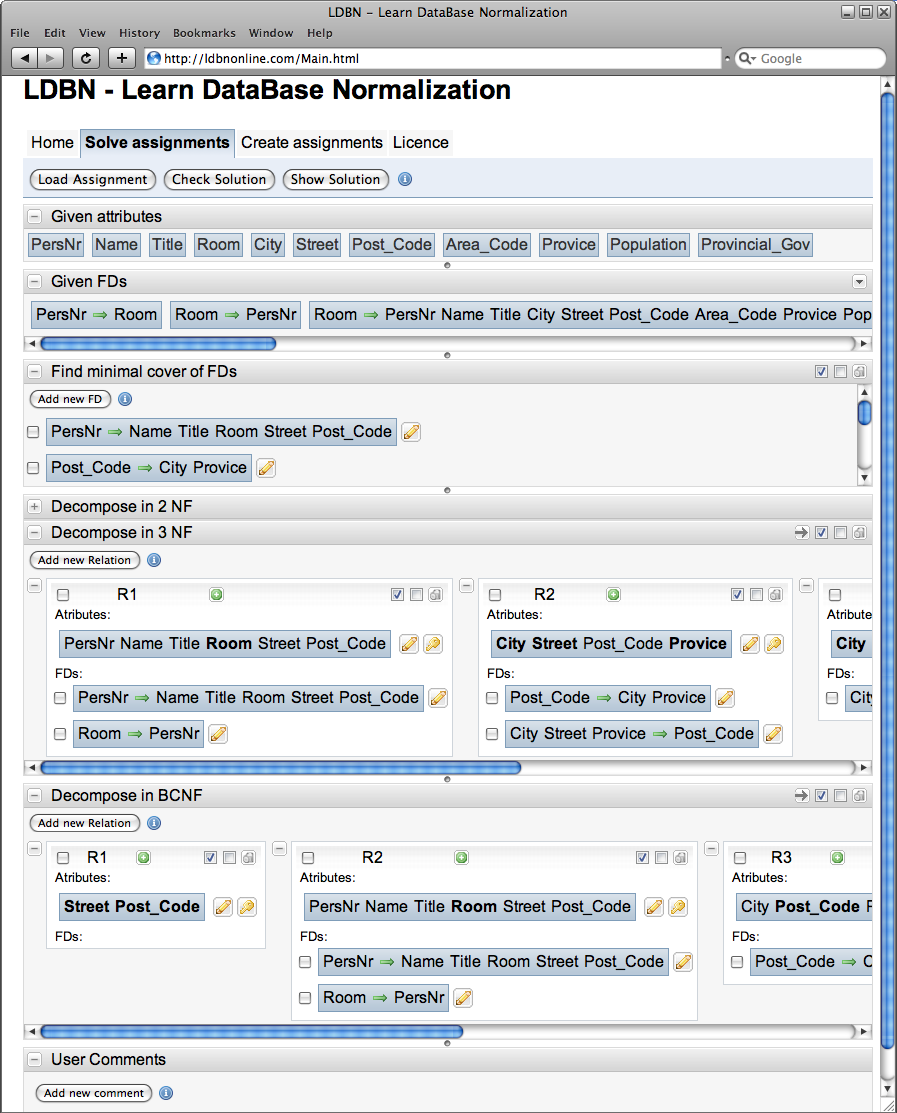
\includegraphics[width=0.8\textwidth]{./img/screen01b.png}
		\caption{LDBN - Solve Assignments Tab}
		\label{fig:screen01}
	\end{center}
\end{figure}

\begin{figure}[h]
	\begin{center}
		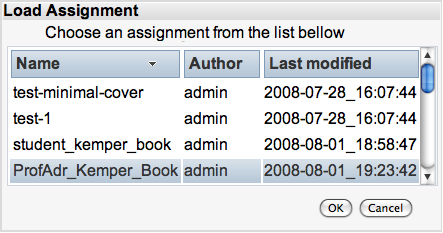
\includegraphics[width=0.6\textwidth]{./img/screen02.png}
		\caption{LDBN - Load Assignments List}
		\label{fig:screen02}
	\end{center}
\end{figure}

Moreover, an assignment consists of a relational schema in First Normal Form (1NF), 
i.e., all the attributes in a single relation and a set of FDs on the attributes. 
After an assignment has been loaded, we require the students to go through the 
following steps in LDBN:
\begin{enumerate}
	\item Determine a minimal cover of the given FDs, also known as canonical cover.
	\item Decompose the relational schema from 1NF into 2NF, 3NF and BCNF. 
	\item Determine a candidate key for each new relation/table. 
\end{enumerate}

Checking a solution is a nonprocedural task, thus the student can start solving
an assignment in a different order. In addition to this,  a partial or complete 
solution can be submitted at any given time by pressing the \textit{Check Solution} button. 
After that the system analyzes the solution by performing the following checks:
\begin{enumerate}
	\item Correctness of the minimal cover of the given FDs. 
	\item Losses join properly for every decomposition.
	\item Dependency preservation for every decomposition.
	\item Correctness of the associated with each relation FDs.
	\item Correctness of the key of each relation.
	\item Correctness of the decomposition, i.e., if the decomposition is really in 2NF, 3NF and BCNF.
\end{enumerate}

\begin{figure}[h]
	\begin{center}
		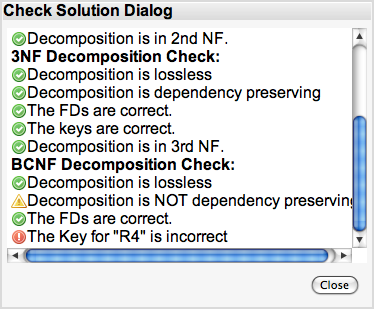
\includegraphics[width=0.6\textwidth]{./img/screen03.png}
		\caption{LDBN - Check Solution Dialog}
		\label{fig:screen03}
	\end{center}
\end{figure}

The user is shown a dialog with the result, and in case of an error the system offers
feedback in form of small textual hints, indicating
where the error might be. Such dialog is shown in Figure~\ref{fig:screen03}. In this case
we can see, that the user has made a correct decomposition for 2NF and 3NF,
but his/her decomposition for BCNF has some errors, namely the key of the relation R4 is
incorrect. The dialog is also showing that the decomposition does not 
satisfy the lossless join property, but in the case of BCNF this
is not allays possible, therefore it is only a warning. 

The concept of assignments is a major
difference between LDBN and the other normalization tools such as the
\textit{Web-based Tool to Enhance Teaching/Learning Database 
Normalization}~\cite{p8} and \textit{The Database Normalization Tool}~\cite{w1}, 
which only provide 
one possible solution (decomposition) to the user, without users having the ability to test 
themselves. In addition, LDBN can be used for checking the correctness of any
arbitrary decomposition, this could be useful for lectures to test handwritten assignments. 
Another major advantage of LDBN over the other tools is the user interface (UI). 
As Frye~\cite{p10} and Dantin~\cite{p9} stated, this is often a
neglected feature, when it comes to educational software. The lack of user-friendly UI 
can often lead to unpopularity of the software among students. An example here could be 
\textit{The Database Normalization Tool}~\cite{w1}. Inputing a relational schema in the program can
take quite sometime, due to the fact that
users have to input every attribute manually using the keyboard and then also 
have to input every FD the same way. This may take several minutes even for small  
assignments. Furthermore, relational schemas cannot be saved for future use like 
in LDBN, and users have to input them again next time. To overcome this slow input of user data, 
LDBN supports Drag and Drop. A feature widely used in desktop
applications, but relatively new to AJAX application such as LDBN. Every attribute
and every FD in LDBN can be dragged and dropped, in order 
to define or modify FDs, key attributes, etc... This ensures a really fast and easy
usage of the tool without the need of a keyboard. It should be mentioned
that inputing attributes the traditional way by tipping them is also supported.

Additional features of LDBN include creating an assignment, which can be done 
only by registered users. This condition is necessary, in order users to be able 
to distinct assignments provided by trusted users, e.g. their database course
lecturers. Registered users have also the ability to leave textual comments 
for every assignment. On the one hand, such
comments ensure that user can easily communicate and share ideas
with each other, and one the other hand, comments could also decrease the amount of workload
for the lecturers in terms of giving an explanation to difficult decomposition.
Such community features are not present in the other two web-based 
normalization tools.

More detailed and formal description of the features of LDBN will be given 
Chapter~\ref{chap:impl}. 


\section{Glossary}
\begin{description}
	\item[2NF, 3NF, BCNF] Second Normal Form, Third Normal Form, Boyce-Codd Normal Form. See Section~\ref{sec:nfintro} for more details.
	\item[AJAX] Asynchronous JavaScript And XML is a group of interrelated web development techniques used for creating interactive web applications, for more details see Section~\ref{sec:ajax}.
	\item[CSS] Cascading Style Sheets is a stylesheet language used to describe the presentation of a document written in HTML.
	\item[DBMS] A database management system (DBMS) is a complex set of software programs that controls the organization, storage, management, and retrieval of data in a database.
	\item[GWT] Google Web Toolkit (GWT) is an open source Java software development framework that allows web developers to create AJAX applications in Java. More details in Section~\ref{sec:gwt}.
	\item[ODBC] Open Database Connectivity (ODBC) provides a standard software API method for using database management systems.
	\item[RPC] Remote procedure call (RPC) is an Inter-process communication technology that allows a computer program to cause a subroutine or procedure to execute in another address space.
	\item[SQL] Structured Query Language, is a computer language designed for the retrieval and management of data in relational database management systems, database schema creation and modification, and database object access control management.
	\item[XMLHttpRequest] is an API that can be used by JavaScript and other web browser scripting languages to transfer asynchronously XML and other text data between a web server and a browser.
\end{description}
